\XtoCBlock{Selector}
\label{block:Selector}
\begin{figure}[H]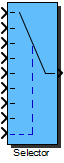
\includegraphics{Selector}\end{figure} 

\begin{XtoCtabular}{Inports}
In0 & Input \#0\tabularnewline
\hline
In1 & Input \#1\tabularnewline
\hline
In2 & Input \#2\tabularnewline
\hline
In3 & Input \#3\tabularnewline
\hline
In4 & Input \#4\tabularnewline
\hline
In5 & Input \#5\tabularnewline
\hline
In6 & Input \#6\tabularnewline
\hline
In7 & Input \#7\tabularnewline
\hline
Select & Input select\tabularnewline
\hline
\end{XtoCtabular}


\begin{XtoCtabular}{Outports}
Out & Selected input signal\tabularnewline
\hline
\end{XtoCtabular}

\subsubsection*{Description:}
Passing through of input signal selected by the select inport:

  Select = 0 (DSP): Out = In0

  Select = 1 (DSP): Out = In1

  ...

  Select = 7 (DSP): Out = In7

% include optional documentation file
\InputIfFileExists{\XcHomePath/Library/General/Doc/Selector_Info.tex}{\vspace{1ex}}{}

\subsubsection*{Implementations:}
\begin{tabular}{l l}
\textbf{FiP8} & 8 Bit Fixed Point Implementation\tabularnewline
\textbf{FiP16} & 16 Bit Fixed Point Implementation\tabularnewline
\textbf{FiP32} & 32 Bit Fixed Point Implementation\tabularnewline
\textbf{Float32} & 32 Bit Floating Point Implementation\tabularnewline
\textbf{Float64} & 64 Bit Floating Point Implementation\tabularnewline
\end{tabular}

\XtoCImplementation{FiP8}
\index{Block ID!400}
\nopagebreak[0]
% Implementation details
\begin{tabular}{l l}
\textbf{Name} & FiP8 \tabularnewline
\textbf{ID} & 400 \tabularnewline
\textbf{Revision} & 1.0 \tabularnewline
\textbf{C filename} & Selector\_FiP8.c \tabularnewline
\textbf{H filename} & Selector\_FiP8.h \tabularnewline
\end{tabular}
\vspace{1ex}

8 Bit Fixed Point Implementation

% Implementation data structure
\XtoCDataStruct{Data Structure:}
\begin{lstlisting}
typedef struct {
     uint16        ID;
     int8          *In0;
     int8          *In1;
     int8          *In2;
     int8          *In3;
     int8          *In4;
     int8          *In5;
     int8          *In6;
     int8          *In7;
     int8          *Select;
     int8          Out;
} SELECTOR_FIP8;
\end{lstlisting}

\ifdefined \AddTestReports
\InputIfFileExists{\XcHomePath/Library/General/Doc/Test_Selector_FiP8.tex}{}{}
\fi
\XtoCImplementation{FiP16}
\index{Block ID!401}
\nopagebreak[0]
% Implementation details
\begin{tabular}{l l}
\textbf{Name} & FiP16 \tabularnewline
\textbf{ID} & 401 \tabularnewline
\textbf{Revision} & 1.0 \tabularnewline
\textbf{C filename} & Selector\_FiP16.c \tabularnewline
\textbf{H filename} & Selector\_FiP16.h \tabularnewline
\end{tabular}
\vspace{1ex}

16 Bit Fixed Point Implementation

% Implementation data structure
\XtoCDataStruct{Data Structure:}
\begin{lstlisting}
typedef struct {
     uint16        ID;
     int16         *In0;
     int16         *In1;
     int16         *In2;
     int16         *In3;
     int16         *In4;
     int16         *In5;
     int16         *In6;
     int16         *In7;
     int8          *Select;
     int16         Out;
} SELECTOR_FIP16;
\end{lstlisting}

\ifdefined \AddTestReports
\InputIfFileExists{\XcHomePath/Library/General/Doc/Test_Selector_FiP16.tex}{}{}
\fi
\XtoCImplementation{FiP32}
\index{Block ID!402}
\nopagebreak[0]
% Implementation details
\begin{tabular}{l l}
\textbf{Name} & FiP32 \tabularnewline
\textbf{ID} & 402 \tabularnewline
\textbf{Revision} & 1.0 \tabularnewline
\textbf{C filename} & Selector\_FiP32.c \tabularnewline
\textbf{H filename} & Selector\_FiP32.h \tabularnewline
\end{tabular}
\vspace{1ex}

32 Bit Fixed Point Implementation

% Implementation data structure
\XtoCDataStruct{Data Structure:}
\begin{lstlisting}
typedef struct {
     uint16        ID;
     int32         *In0;
     int32         *In1;
     int32         *In2;
     int32         *In3;
     int32         *In4;
     int32         *In5;
     int32         *In6;
     int32         *In7;
     int8          *Select;
     int32         Out;
} SELECTOR_FIP32;
\end{lstlisting}

\ifdefined \AddTestReports
\InputIfFileExists{\XcHomePath/Library/General/Doc/Test_Selector_FiP32.tex}{}{}
\fi
\XtoCImplementation{Float32}
\index{Block ID!403}
\nopagebreak[0]
% Implementation details
\begin{tabular}{l l}
\textbf{Name} & Float32 \tabularnewline
\textbf{ID} & 403 \tabularnewline
\textbf{Revision} & 1.0 \tabularnewline
\textbf{C filename} & Selector\_Float32.c \tabularnewline
\textbf{H filename} & Selector\_Float32.h \tabularnewline
\end{tabular}
\vspace{1ex}

32 Bit Floating Point Implementation

% Implementation data structure
\XtoCDataStruct{Data Structure:}
\begin{lstlisting}
typedef struct {
     uint16        ID;
     float32       *In0;
     float32       *In1;
     float32       *In2;
     float32       *In3;
     float32       *In4;
     float32       *In5;
     float32       *In6;
     float32       *In7;
     int8          *Select;
     float32       Out;
} SELECTOR_FLOAT32;
\end{lstlisting}

\ifdefined \AddTestReports
\InputIfFileExists{\XcHomePath/Library/General/Doc/Test_Selector_Float32.tex}{}{}
\fi
\XtoCImplementation{Float64}
\index{Block ID!404}
\nopagebreak[0]
% Implementation details
\begin{tabular}{l l}
\textbf{Name} & Float64 \tabularnewline
\textbf{ID} & 404 \tabularnewline
\textbf{Revision} & 1.0 \tabularnewline
\textbf{C filename} & Selector\_Float64.c \tabularnewline
\textbf{H filename} & Selector\_Float64.h \tabularnewline
\end{tabular}
\vspace{1ex}

64 Bit Floating Point Implementation

% Implementation data structure
\XtoCDataStruct{Data Structure:}
\begin{lstlisting}
typedef struct {
     uint16        ID;
     float64       *In0;
     float64       *In1;
     float64       *In2;
     float64       *In3;
     float64       *In4;
     float64       *In5;
     float64       *In6;
     float64       *In7;
     int8          *Select;
     float64       Out;
} SELECTOR_FLOAT64;
\end{lstlisting}

\ifdefined \AddTestReports
\InputIfFileExists{\XcHomePath/Library/General/Doc/Test_Selector_Float64.tex}{}{}
\fi
